\documentclass[tikz, 11pt]{standalone}
%
\usetikzlibrary{calc}
\usepackage{graphicx}
\usepackage[scaled=0.92]{helvet}%3.75
\renewcommand{\familydefault}{\sfdefault}
\usepackage{textcomp}
%
\graphicspath{{Cropped/}}
%
\newlength{\PicWidth}
\newlength{\VSep}
\newlength{\HSep}
\newlength{\LabelSep}
%
\begin{document}
	%	
	\setlength{\PicWidth}{2.8cm}
	\setlength{\VSep}{1ex}
	\setlength{\HSep}{1.5ex}
	\setlength{\LabelSep}{0.5ex}
	%	
	\scriptsize % font size
	%
	\graphicspath{{photos/}}
	\begin{tikzpicture}[every node/.style={inner sep=0ex},%
						MediaLabel/.style={font={\bfseries}, align=left}]
		%
		% YPD
		\path (0,0) node (YPD) {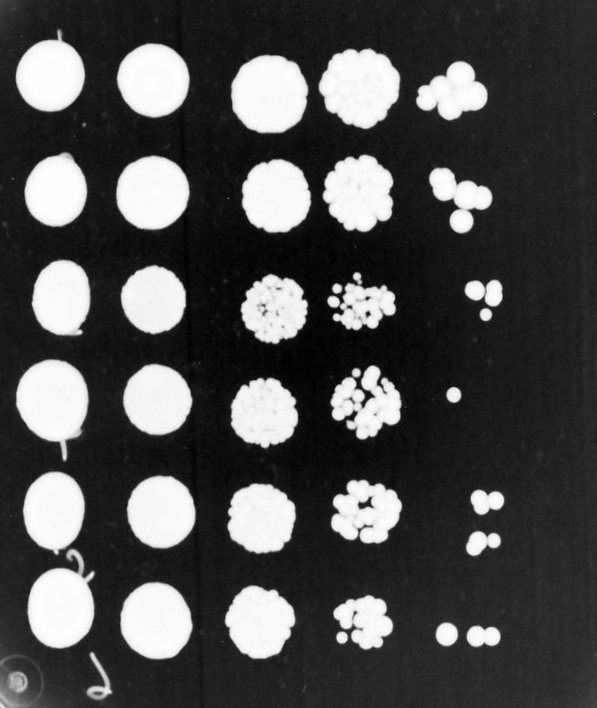
\includegraphics[width=\PicWidth]{YPD.jpg}};
		% strains
		\pgfmathsetmacro{\Start}{0.12}
		\pgfmathsetmacro{\Sep}{0.155}
		\foreach[count=\i] \strain in {\textit{fun30$\Delta$}, \textit{sgs1$\Delta$ fun30$\Delta$}, \textit{exo1$\Delta$ sgs1$\Delta$ fun30$\Delta$}, \textit{exo1$\Delta$ sgs1$\Delta$ fun30$\Delta$}, \textit{exo1$\Delta$ sgs1$\Delta$}, \textit{exo1$\Delta$ sgs1$\Delta$}}{
			\pgfmathsetmacro{\x}{\Start+(\i-1)*\Sep}
			\path ($(YPD.north west)!\x!(YPD.south west)$) node[xshift=-\LabelSep, anchor=east] {\strain};
		}
		%
		% CPT
		\path (YPD.east) ++(\HSep,0) node[anchor=west] (CPT) {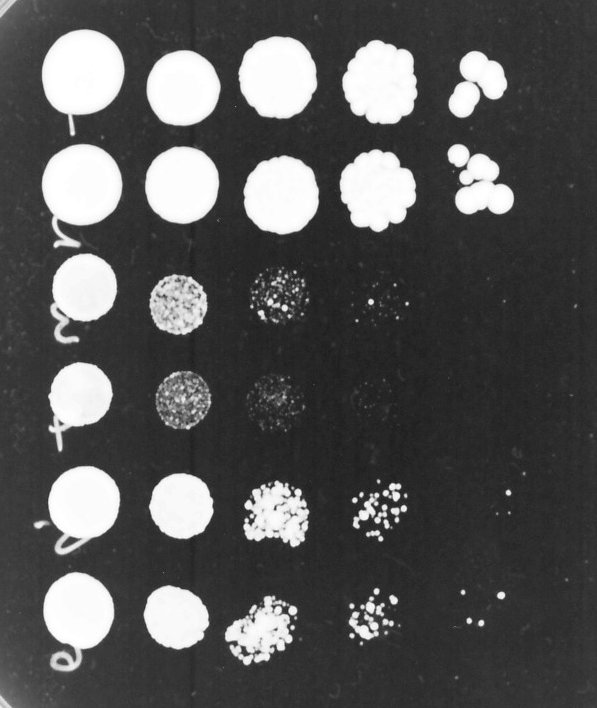
\includegraphics[width=\PicWidth]{CPT.jpg}};
		%
		% add top Rap labels
		\path (YPD.north) ++(0,\LabelSep) node[anchor=south, MediaLabel] {YPD\vphantom{$\mu$g}};
		\path (CPT.north) ++(0,\LabelSep) node[anchor=south, MediaLabel] {YPD + 0.25 $\mu$g/ml CPT};
		%
	\end{tikzpicture}
	%
\end{document}